\documentclass[spanish,a4paper,11pt,twoside]{report}

%%%%%%%%%%%%%%%%%%%%%%%%%%%%%%%%%%%%%%%%%%%%%%%%%%%%%%%%%%%%%%%%%%%%%%%%%%%%%%%
\usepackage[dvips]{graphicx}
\usepackage[dvips]{epsfig}
\usepackage[utf8]{inputenc}
\usepackage[english]{babel}
\usepackage{alltt}
\usepackage{templates/algorithm}
\usepackage{templates/algorithmic}
\usepackage{templates/multirow}

%%%%%%%%%%%%%%%%%%%%%%%%%%%%%%%%%%%%%%%%%%%%%%%%%%%%%%%%%%%%%%%%%%%%%%%%%%%%%%%

\newcommand{\SONY}{{\sc Sony}}
\newcommand{\MICROSOFT}{{\sc Microsoft}}
\newcommand{\GCC}{\textsf{\textsc{G}CC}}
\newcommand{\INTEL}{\textsf{\textsc{I}ntel}}

%%% Traducimos el pseudocodigo
\renewcommand{\algorithmicwhile}{\textbf{mientras}}
\renewcommand{\algorithmicend}{\textbf{fin}}
\renewcommand{\algorithmicdo}{\textbf{hacer}}
\renewcommand{\algorithmicif}{\textbf{si}}
\renewcommand{\algorithmicthen}{\textbf{entonces}}
\renewcommand{\algorithmicrepeat}{\textbf{repetir}}
\renewcommand{\algorithmicuntil}{\textbf{hasta que}}
\renewcommand{\algorithmicelse}{\textbf{en otro caso}}
\renewcommand{\algorithmicfor}{\textbf{para}}

%\newcommand{\RETURN}{\textbf{retornar} }
\newcommand{\RET}{\STATE \textbf{retornar} }
\newcommand{\TO}{\textbf{hasta} }
\newcommand{\AND}{\textbf{y} }
\newcommand{\OR}{\textbf{o} }

%%%%%%%%%%%%%%%%% Creamos un entorno para listar código fuente %%%%%%%%%%%%%%%
\newenvironment{sourcecode}
{\begin{list}{}{\setlength{\leftmargin}{1em}}\item\scriptsize\bfseries}
{\end{list}}

\newenvironment{littlesourcecode}
{\begin{list}{}{\setlength{\leftmargin}{1em}}\item\tiny\bfseries}
{\end{list}}

\newenvironment{summary}
{\par\noindent\begin{center}\textbf{Abstract}\end{center}\begin{itshape}\par\noindent}
{\end{itshape}}

\newenvironment{keywords}
{\begin{list}{}{\setlength{\leftmargin}{1em}}\item[\hskip\labelsep \bfseries Keywords:]}
{\end{list}}

\newenvironment{palabrasClave}
{\begin{list}{}{\setlength{\leftmargin}{1em}}\item[\hskip\labelsep \bfseries Palabras clave:]}
{\end{list}}


%%%%%%%%%%%%%%%%%%%%%%%%%%%%%%%%%%%%%%%%%%%%%%%%%%%%%%%%%%%%%%%%%%%%%%%%%%%%%%%
% Format
%%%%%%%%%%%%%%%%%%%%%%%%%%%%%%%%%%%%%%%%%%%%%%%%%%%%%%%%%%%%%%%%%%%%%%%%%%%%%%%

%%\topmargin -4 mm
%\topmargin -21 mm
%\headheight 10 mm
%\headsep 10 mm

%\textheight 229 mm
%\textheight 246 mm

%\oddsidemargin -5.4 mm
%\evensidemargin -5.4 mm
\oddsidemargin 5 mm
\evensidemargin 5 mm

%\oddsidemargin -3 mm
%\evensidemargin -3 mm

%\textwidth 17 cm
\textwidth 15 cm
%\columnsep 10 mm

\input{amssym.def}

%%%%%%%%%%%%%%%%%%%%%%%%%%%%%%%%%%%%%%%%%%%%%%%%%%%%%%%%%%%%%%%%%%%%%%%%%%%%%%%

\begin{document}

%%%%%%%%%%%%%%%%%%%%%%%%%%%%%%%%%%%%%%%%%%%%%%%%%%%%%%%%%%%%%%%%%%%%%%%%%%%%%%%
% First Page 
%%%%%%%%%%%%%%%%%%%%%%%%%%%%%%%%%%%%%%%%%%%%%%%%%%%%%%%%%%%%%%%%%%%%%%%%%%%%%%%

\pagestyle{empty}
\thispagestyle{empty}


\newcommand{\HRule}{\rule{\linewidth}{1mm}}
\setlength{\parindent}{0mm}
\setlength{\parskip}{0mm}
\vspace*{\stretch{1}}

\begin{center}
\includegraphics[width=0.2\textwidth]{images/logotipo-secundario-ULL}\\[0.25cm]
\end{center}

\HRule
\begin{center}
        {\Huge Proyecto de la asignatura Computacion Avanzada } \\[2.5mm] 
        {\Huge Título del Artículo :   Solving simulation optimization problems on grid computing systems
} \\[5mm]

        {\Large Autor : YOUSEF RAJAEITABRIZI} \\[10mm]

        {\em Computación Avanzada} \\[5mm]
        Lenguajes y Sistemas Informáticos \\[5mm]
        Escuela Técnica Superior de Ingeniería y Tecnología \\[5mm]
        
        Universidad de La Laguna \\
\end{center}
\HRule
\vspace*{\stretch{2}}
\begin{center}
  La Laguna, \today 
\end{center}

%%%%%%%%%%%%%%%%%%%%%%%%%%%%%%%%%%%%%%%%%%%%%%%%%%%%%%%%%%%%%%%%%%%%%%%%%%%%%%%
\begin{abstract}
{\em

%El objetivo de este trabajo ha sido ....
%
%bla, bla, bla
%
%bla, bla, bla
%
%bla, bla, bla
The main novelty of this paper is the use of grid computing for solving (iterative) simulation optimization problems.
The global guidance system of the search method is asked to reach and select a near-optimum solution in a relatively short time; it may have a significant improvement with computing resources that work in parallel as much as possible, by exploring larger subsets of feasible configurations of the model.
 The policy designed to arrange the exploration is a crucial part of the whole algorithm to be designed for the optimum seeking problem at hand.
Moreover, at an inner level, a specific subset of computing resources may have their own capability of:

• parallel execution of stochastic simulation;

• parallel replication of stochastic simulation to get an adequate level of statistical confidence on the performance

indices of the assigned configurations, during the (outer) optimization process.

}

\begin{palabrasClave}
Queuing model :One way to mostrate setting of ships.
\end{palabrasClave}

\end{abstract}
%%%%%%%%%%%%%%%%%%%%%%%%%%%%%%%%%%%%%%%%%%%%%%%%%%%%%%%%%%%%%%%%%%%%%%%%%%%%%%%

%%%%%%%%%%%%%%%%%%%%%%%%%%%%%%%%%%%%%%%%%%%%%%%%%%%%%%%%%%%%%%%%%%%%%%%%%%%%%%%
\newpage{\pagestyle{empty}\cleardoublepage}

\pagestyle{myheadings} %my head defined by markboth or markright
% No funciona bien \markboth sin "twoside" en \documentclass, pero al
% ponerlo se dan un mont�n de errores de underfull \vbox, con lo que no se
% ha puesto.
\markboth{YOUSEF RAJAEITABRIZI}{Solving simulation optimization problems on grid computing systems}

%%%%%%%%%%%%%%%%%%%%%%%%%%%%%%%%%%%%%%%%%%%%%%%%%%%%%%%%%%%%%%%%%%%%%%%%%%%%%%%
%Numeracion en romanos
\renewcommand{\thepage}{\roman{page}}
\setcounter{page}{1}


%\tableofcontents

%%%%%%%%%%%%%%%%%%%%%%%%%%%%%%%%%%%%%%%%%%%%%%%%%%%%%%%%%%%%%%%%%%%%%%%%%%%%%%%

%\listoffigures

%%%%%%%%%%%%%%%%%%%%%%%%%%%%%%%%%%%%%%%%%%%%%%%%%%%%%%%%%%%%%%%%%%%%%%%%%%%%%%%

%\listoftables

%%%%%%%%%%%%%%%%%%%%%%%%%%%%%%%%%%%%%%%%%%%%%%%%%%%%%%%%%%%%%%%%%%%%%%%%%%%%%%%
%\newpage{\pagestyle{empty}\cleardoublepage}

%%%%%%%%%%%%%%%%%%%%%%%%%%%%%%%%%%%%%%%%%%%%%%%%%%%%%%%%%%%%%%%%%%%%%%%%%%%%%%%
%Numeracion a partir del capitulo I
\renewcommand{\thepage}{\arabic{page}}
\setcounter{page}{1}

\setlength{\parindent}{5mm}

%%%%%%%%%%%%%%%%%%%%%%%%%%%%%%%%%%%%%%%%%%%%%%%%%%%%%%%%%%%%%%%%%%%%%%%%%%%%%%%
\chapter{Motivación y objetivos}
\label{chapter:obj}

%%%%%%%%%%%%%%%%%%%%%%%%%%%%%%%%%%%%%%%%%%%%%%%%%%%%%%%%%%%%%%%%%%%%%%%%%%%%%
% Chapter 1: Queuing model and mathematical formulation
%%%%%%%%%%%%%%%%%%%%%%%%%%%%%%%%%%%%%%%%%%%%%%%%%%%%%%%%%%%%%%%%%%%%%%%%%%%%%%%
In the sequel we illustrate the proposed queuing model in which we eliminate some details from the model description of Legato and Mazza [12] because they are not significant for the purpose of this paper.
We assume that the occurrence of a delay-time spent at roadstead by an incoming vessel, due to lack of berth slots, is represented as a special case of the phase type Cox’s distribution. This assumption can be accepted for the following considerations. Usually, an incoming vessel receives almost immediately the required slots for berthing. In this case, with a very high probability (p), the elapsing interval from ‘‘arrival to port’’ and ‘‘berthing time completion’’ results in a very short time (l1, on average), due to the relatively fast operations for vessel positioning along the berth. With a very low probability (1  p), an arrived vessel is delayed at roadstead due to unavailability of the required berth slots: once this happens, then a very long interval (l1 + l2, on average) elapses from ‘‘arrival to port’’ and ‘‘berthing time’’ (Fig. 1). An illustrative example based on real data referred to a shipping company at Gioia Tauro port, in September 2002, is given in Fig. 2. Fig.
In the sequel we illustrate the proposed queuing model in which we eliminate some details from the model
description of Legato and Mazza [12] because they are not significant for the purpose of this paper.
We assume that the occurrence of a delay-time spent at roadstead by an incoming vessel, due to lack of
berth slots, is represented as a special case of the phase type Cox’s distribution. This assumption can be
accepted for the following considerations. Usually, an incoming vessel receives almost immediately the
required slots for berthing. In this case, with a very high probability (p), the elapsing interval from ‘‘arrival
to port’’ and ‘‘berthing time completion’’ results in a very short time (l1, on average), due to the relatively
fast operations for vessel positioning along the berth. With a very low probability (1  p), an arrived vessel
is delayed at roadstead due to unavailability of the required berth slots: once this happens, then a very long
interval (l1 + l2, on average) elapses from ‘‘arrival to port’’ and ‘‘berthing time’’ (Fig. 1). An illustrative
example based on real data referred to a shipping company at Gioia Tauro port, in September 2002, is given
in Fig. 2.


%---------------------------------------------------------------------------------
%\section{Sección Uno}
%\label{1:sec:1}
 % Primer párrafo de la primera sección.


%---------------------------------------------------------------------------------
%\section{Sección Dos}
%\label{1:sec:2}
%  Primer párrafo de la segunda sección.

%\begin{itemize}
%  \item Item 1
%  \item Item 2
%  \item Item 3
%\end{itemize}


%""""""""""""""""""""""""""""""""""""""""""""""""""""""""""""""""""""""""""""""
\begin{center}
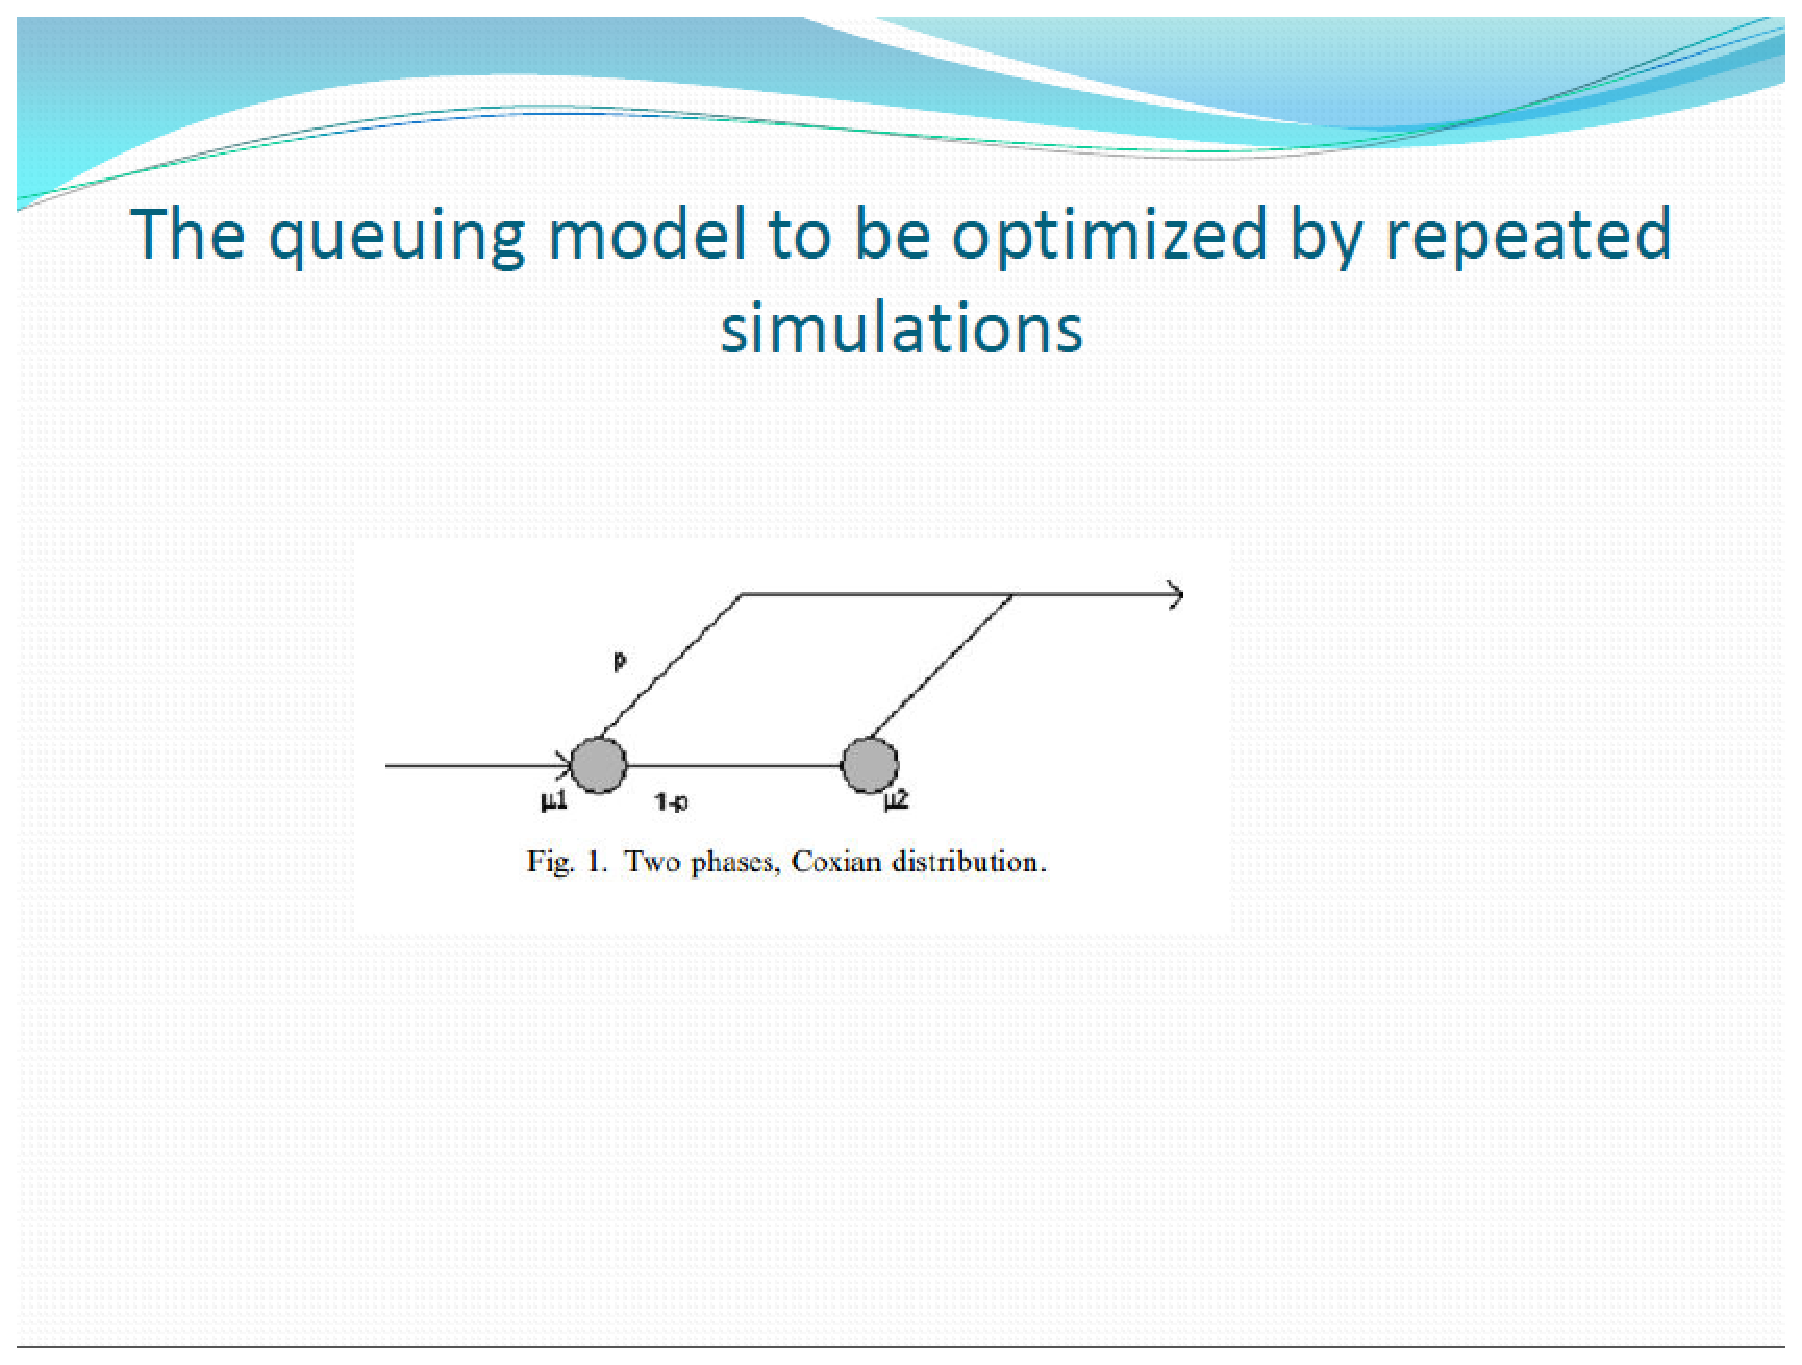
\includegraphics[width=1\textwidth]{images/pic4.eps}\\[0.25cm]
\end{center}

%%%%%%%%%%%%%%%%%%%%%%%%%%%%%%%%%%%%%%%%%%%%%%%%%%%%%%%%%%%%%%%%%%%%%%%%%%%%%%%
\chapter{Fundamentos teóricos}
\label{chapter:teo}

%%%%%%%%%%%%%%%%%%%%%%%%%%%%%%%%%%%%%%%%%%%%%%%%%%%%%%%%%%%%%%%%%%%%%%%%%%%%%%%
% Chapter 2: The simulation optimization model requisitos : 
%%%%%%%%%%%%%%%%%%%%%%%%%%%%%%%%%%%%%%%%%%%%%%%%%%%%%%%%%%%%%%%%%%%%%%%%%%%%%%%

%++++++++++++++++++++++++++++++++++++++++++++++++++++++++++++++++++++++++++++++
In the berth planning problem, we should answer the following questions:
 how many segments do we organize for active shipping services? 
 how many cranes – out of the total, fixed, number of available ones  do we allocate for each of the organized segments? 
 to which segment do we forward incoming vessels, provided that we may base this decision on some suitable attributes shared by any given subset of the active services? 
Answers to these questions are provided by the simulation optimization approach.
3.2. Grid enabled versions for the SARP algorithm
With the aim of developing grid versions of the SARP algorithm described above (in the sequel G-SARP),
we have adopted a master/worker approach [16,4,19].
Let p be the number of workers. At iteration k, the master creates p + 1 perturbations of a same configuration
of the system (i.e. p + 1 neighbours of the current solution), keeps for itself the first generated configuration
to be estimated and sends the others to the workers (one configuration for each worker). Each processor,
including the master, must decide if its own configuration can be accepted or not. If a processor accepts its
own solution (according to the acceptance criterion of SARP), then sends it to the master. If the master has
new solutions to examine, it selects the next configuration, otherwise it keeps the old one. There are different
rules for selection; for example, the master can choose the configuration with the best estimated performance
(best strategy) or it can make a random choice (random strategy). We have implemented both, and we present in
 4 and 5 illustrate the master and the worker process, respectively. In
our computational scheme, different workers carry out simulation experiments on different neighbours.
In other words, through the grid platform, we explore a richer neighbourhood at each iteration and perform
a more effective procedure for optimization via simulation; whereas SARP simply uses a simulated
annealing routine, G-SARP integrates simulated annealing with a sampling routine. To this purpose, a point
of synchronization between the master and the workers is needed to evaluate the results of sampling, update
current solution and redefine the neighbours.
Our procedure has been tuned as follows.
%++++++++++++++++++++++++++++++++++++++++++++++++++++++++++++++++++++++++++++++

%\section{Primer apartado del segundo capítulo}
%\label{2:sec:1}
%  Primer párrafo de la primera sección.

%\section{Segundo apartado del segundo capítulo}
%\label{2:sec:2}
%  Primer párrafo de la segunda sección.


%""""""""""""""""""""""""""""""""""""""""""""""""""""""""""""""""""""""""""""""
\begin{center}
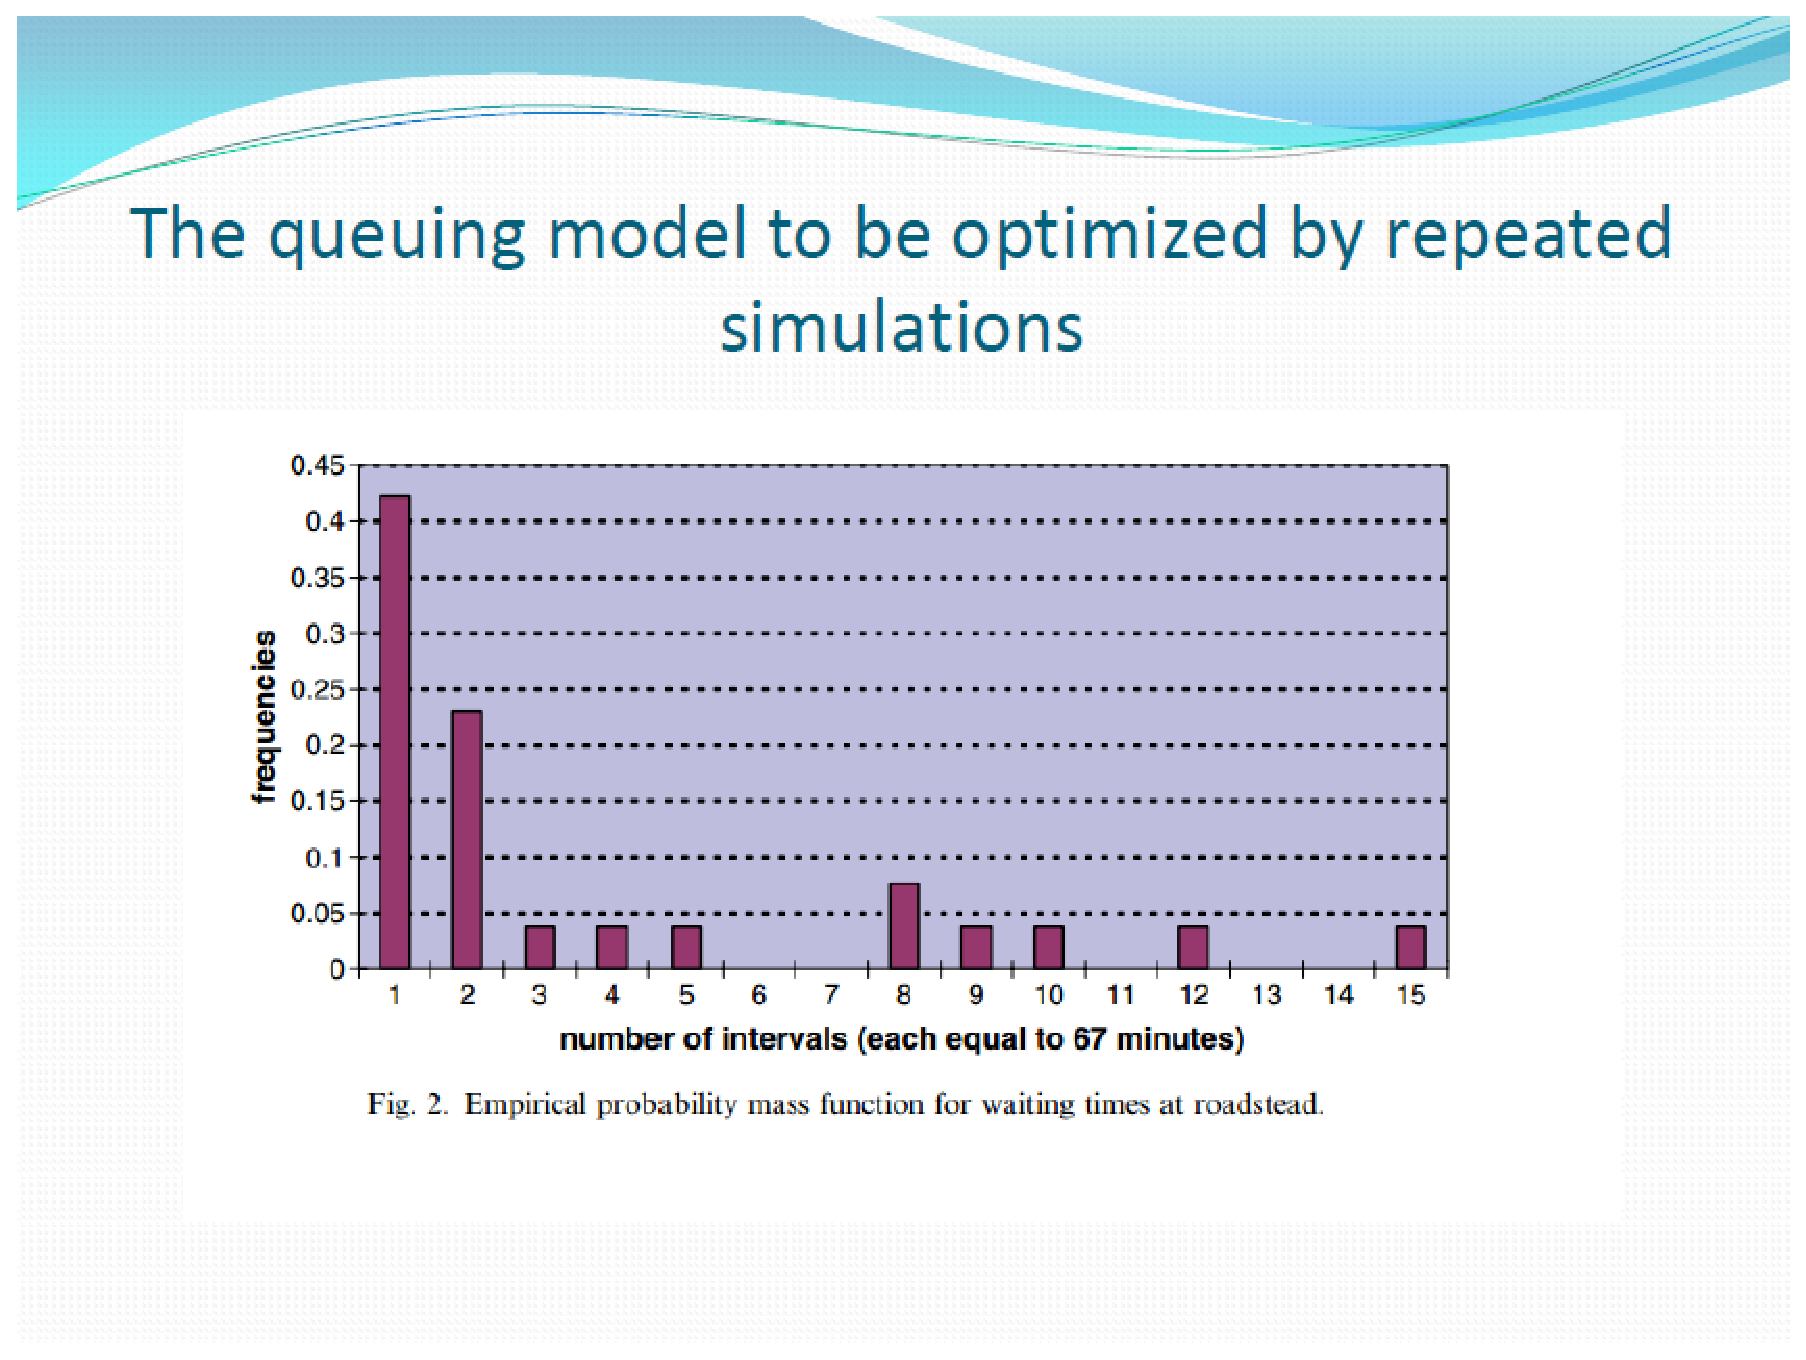
\includegraphics[width=1\textwidth]{images/pic5.eps}\\[0.25cm]
\end{center}
%""""""""""""""""""""""""""""""""""""""""""""""""""""""""""""""""""""""""""""""

%%%%%%%%%%%%%%%%%%%%%%%%%%%%%%%%%%%%%%%%%%%%%%%%%%%%%%%%%%%%%%%%%%%%%%%%%%%%%%%
\chapter{Procedimiento experimental}
\label{chapter:exp}

%%%%%%%%%%%%%%%%%%%%%%%%%%%%%%%%%%%%%%%%%%%%%%%%%%%%%%%%%%%%%%%%%%%%%%%%%%%%%%%
% Chapter 3: Computational experiments 
%%%%%%%%%%%%%%%%%%%%%%%%%%%%%%%%%%%%%%%%%%%%%%%%%%%%%%%%%%%%%%%%%%%%%%%%%%%%%%%

In our master/worker approach, the master keeps track of the pool of configurations dispatched to the workers. Thus, whenever a worker is subjected to crashes, the master can reassign the same configuration to another worker. On the contrary, whenever the master node crashes there is no way to recover the instantaneous state of the computational procedure. To react at the occurrence of a master crash, we have implemented a periodic checkpoint. Specifically, at a sequence of suitable time points when no messages are in transit back from any worker, the value of the best feasible solution up to current time is recorded and, also, the list of the ‘‘latest’’ parallel configurations that have been dispatched to the workers is saved in a file system. In such a way the G-SARP algorithm can be restarted from latest perturbation step.

%++++++++++++++++++++++++++++++++++++++++++++++++++++++++++++++++++++++++++++++
%\section{Descripción de los experimentos}
%\label{3:sec:1}

%bla, bla, etc. 

%++++++++++++++++++++++++++++++++++++++++++++++++++++++++++++++++++++++++++++++
%\section{Descripción del material}
%\label{3:sec:2}

%bla, bla, etc. 


%++++++++++++++++++++++++++++++++++++++++++++++++++++++++++++++++++++++++++++++
%\section{Resultados obtenidos}
%\label{3:sec:3}

%bla, bla, etc. 


%------------------------------------------------------------------------------
%\begin{figure}[!th]
%\begin{center}
%\includegraphics[width=0.50\textwidth]{images/figura1.eps}
%\caption{Ejemplo de figura}
%\label{fig:1}
%\end{center}
%\end{figure}
%------------------------------------------------------------------------------


%------------------------------------------------------------------------------
%\input{tables/table.tex}
%------------------------------------------------------------------------------

%++++++++++++++++++++++++++++++++++++++++++++++++++++++++++++++++++++++++++++++
\section{ Computational experiments}
\label{3:sec:4}

%bla, bla, etc. 


The potential benefit of grid computing has been evaluated against the combinatorial number of queuing
network configurations to be simulated by the workers. To get an idea of this number in a possible scenario’s
analysis, consider the case of Gioia Tauro port cited in Section 2. Once the terminal manager has fixed ‘‘n’’
berthing points (about 10–12) along the quay (3.3 km long) then he has to displace all the available berth
cranes (15–18 units, mounted on rail) along the berthing positions and, moreover, he has to assign each shipping
service (out of more than 20) to its own berthing point.
The grid platform used in the experiments is a portion of the campus grid at University of Calabria characterized
by a network of super-computers, physically located in different centres within the campus area. The
heterogeneous computing resources used are described in Table 1.
Wall-clock time experienced by us to get a satisfactory solution for this problem is of the order of some
hours. Hence, considering that in a real organisational framework simulation optimization problems are
expected to run on a network of slower workstations or even PCs, one may recognize that grid computing
appears to be the unique cost effective tool which can provide proper solutions to decision problems in a reasonable
amount of time for the terminal manager.
The efficient and transparent execution  is supported by, a complete implementation
of the MPI-1 standard that uses the Globus Toolkit collection of software components (services). In particular,
the  command of the Globus Toolkit activates the execution of  programs to
manage process execution, access to remote files and so on. We have observed that MPI program can be performed
without any changes, as in a common parallel program.
Using a master/worker approach with a well structured procedure, like G-SARP, it seems natural to ensure
a fault tolerant computing [9] by the common practice of checkpoints. By considering the problem of the node
crash, the programmer is asked to implement a policy to manage with two different types of crashes: a crash of
the master node, and a crash of a worker node. Our technique for tolerating failure of one or more workers is
based on a simple idea. In our master/worker approach, the master keeps track of the pool of configurations
dispatched to the workers. Thus, whenever a worker is subjected to crashes, the master can reassign the same
configuration to another worker. On the contrary,
%""""""""""""""""""""""""""""""""""""""""""""""""""""""""""""""""""""""""""""""
\begin{center}
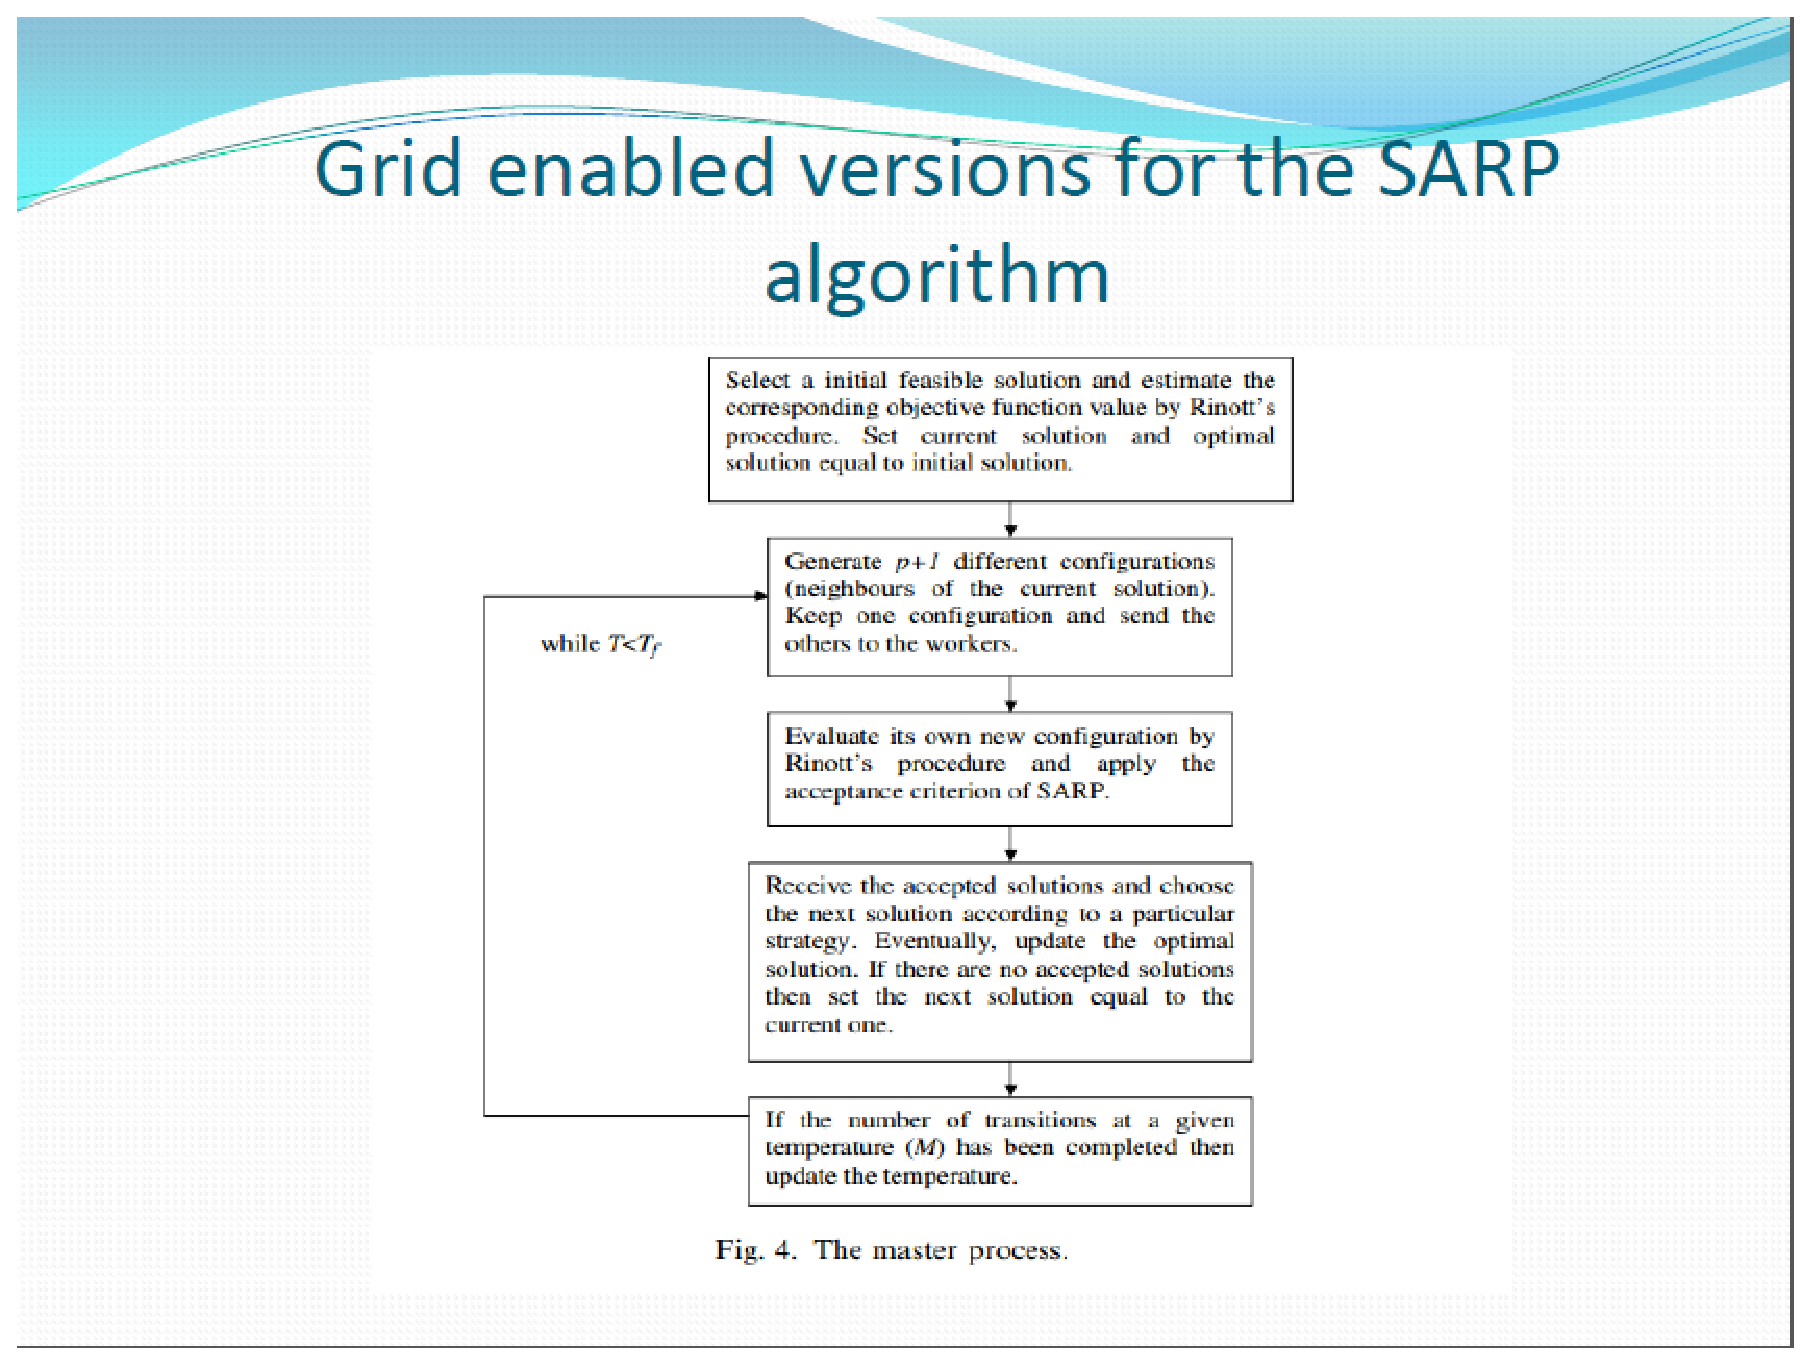
\includegraphics[width=1\textwidth]{images/pic9.eps}\\[0.25cm]
\end{center}
%""""""""""""""""""""""""""""""""""""""""""""""""""""""""""""""""""""""""""""""
%""""""""""""""""""""""""""""""""""""""""""""""""""""""""""""""""""""""""""""""
\begin{center}
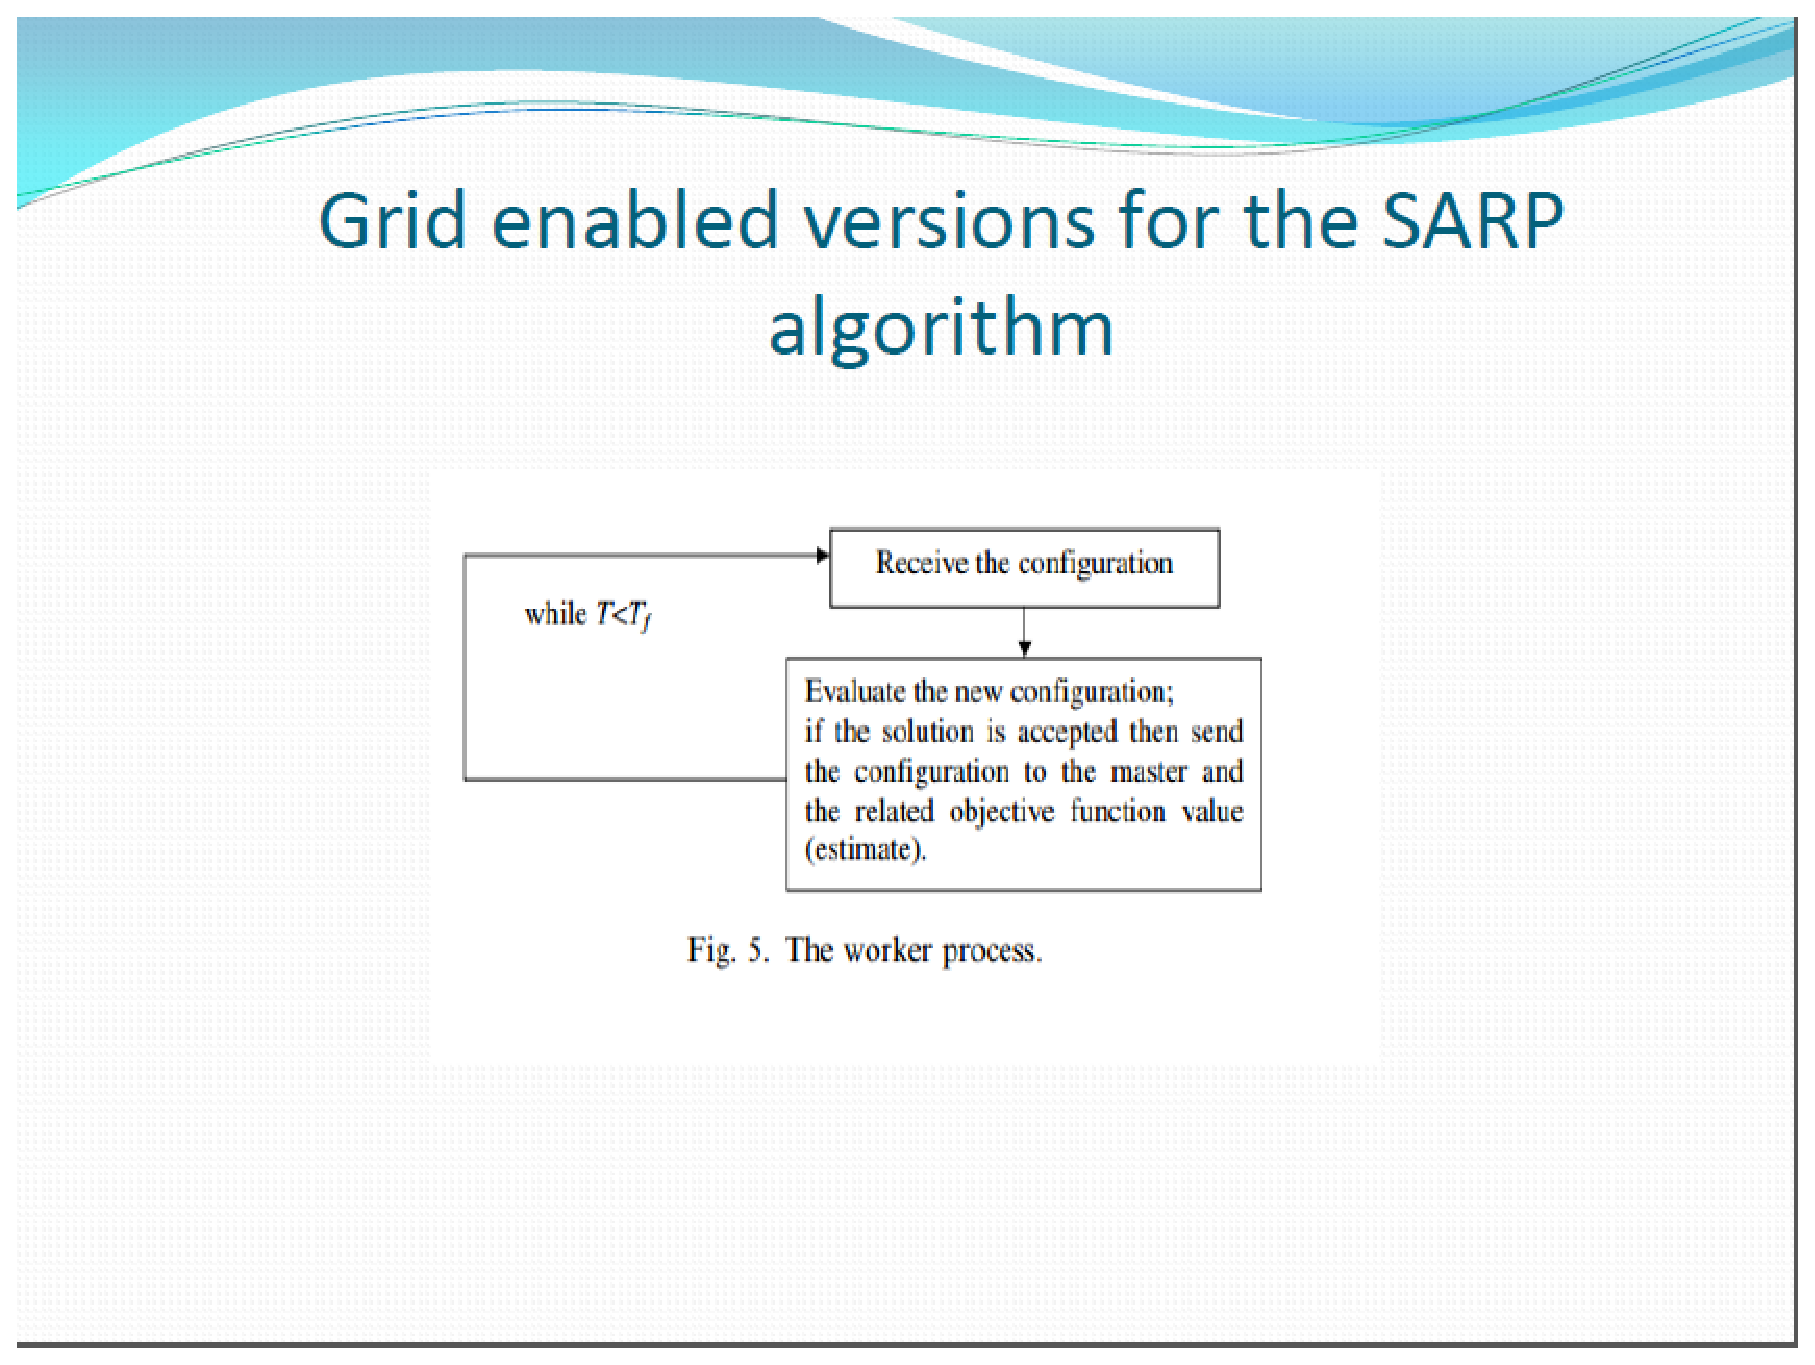
\includegraphics[width=1\textwidth]{images/pic10.eps}\\[0.25cm]
\end{center}
%%%%%%%%%%%%%%%%%%%%%%%%%%%%%%%%%%%%%%%%%%%%%%%%%%%%%%%%%%%%%%%%%%%%%%%%%%%%%%%

%""""""""""""""""""""""""""""""""""""""""""""""""""""""""""""""""""""""""""""""
%%%%%%%%%%%%%%%%%%%%%%%%%%%%%%%%%%%%%%%%%%%%%%%%%%%%%%%%%%%%%%%%%%%%%%%%%%%%%%%
\chapter{Conclusiones}
\label{chapter:conclusiones}

%%%%%%%%%%%%%%%%%%%%%%%%%%%%%%%%%%%%%%%%%%%%%%%%%%%%%%%%%%%%%%%%%%%%%%%%%%%%%
% Chapter 4: Conclusion and future work
%%%%%%%%%%%%%%%%%%%%%%%%%%%%%%%%%%%%%%%%%%%%%%%%%%%%%%%%%%%%%%%%%%%%%%%%%%%%%%%

We have designed and implemented on a grid platform a simulation optimization algorithm that requires a limited amount of communication and a minimal synchronization among computing resources. It could be used for a cost-effective solution of logistics decision problems at seaport container terminals. Numerical evidence shows that as the number of workers increases, the quality of the final solution improves. A crucial role is played by the optimal compromise between searching the entire feasible region (exploration) and locally searching promising sub-regions (exploitation).
Numerical results are presented to compare the quality of solutions for different number of processors
employed, taking as reference 14 test problems which differ in the following parameters: profit values, number
of shipping services, maximum number of berth segments and budget. In particular, simulation runs have been
executed without resorting to any parallel computing capability, even though this could be implemented
according to the guidelines in Section 4. Here we concentrate on isolating the trend of improvement of the
neighbourhood exploration algorithm (simulated annealing with sampling) as the number of workers
increases, under both the alternative strategies (best and random) for updating the current solution. The
improvement of the quality of the final solution appears more significant as the complexity of the test problem
increases. In this case, the practical possibility of exploring a richer sub-region of the solution space increases
substantially by using a larger number of workers. Hence, an interesting research issue raised by the master–
worker framework is that of finding the most effective balance between the explorative work carried out by
the workers (all together) on an intelligent partition of the entire feasible region and the exploitative work
by one worker within one sub-region.

%""""""""""""""""""""""""""""""""""""""""""""""""""""""""""""""""""""""""""""""
\begin{center}
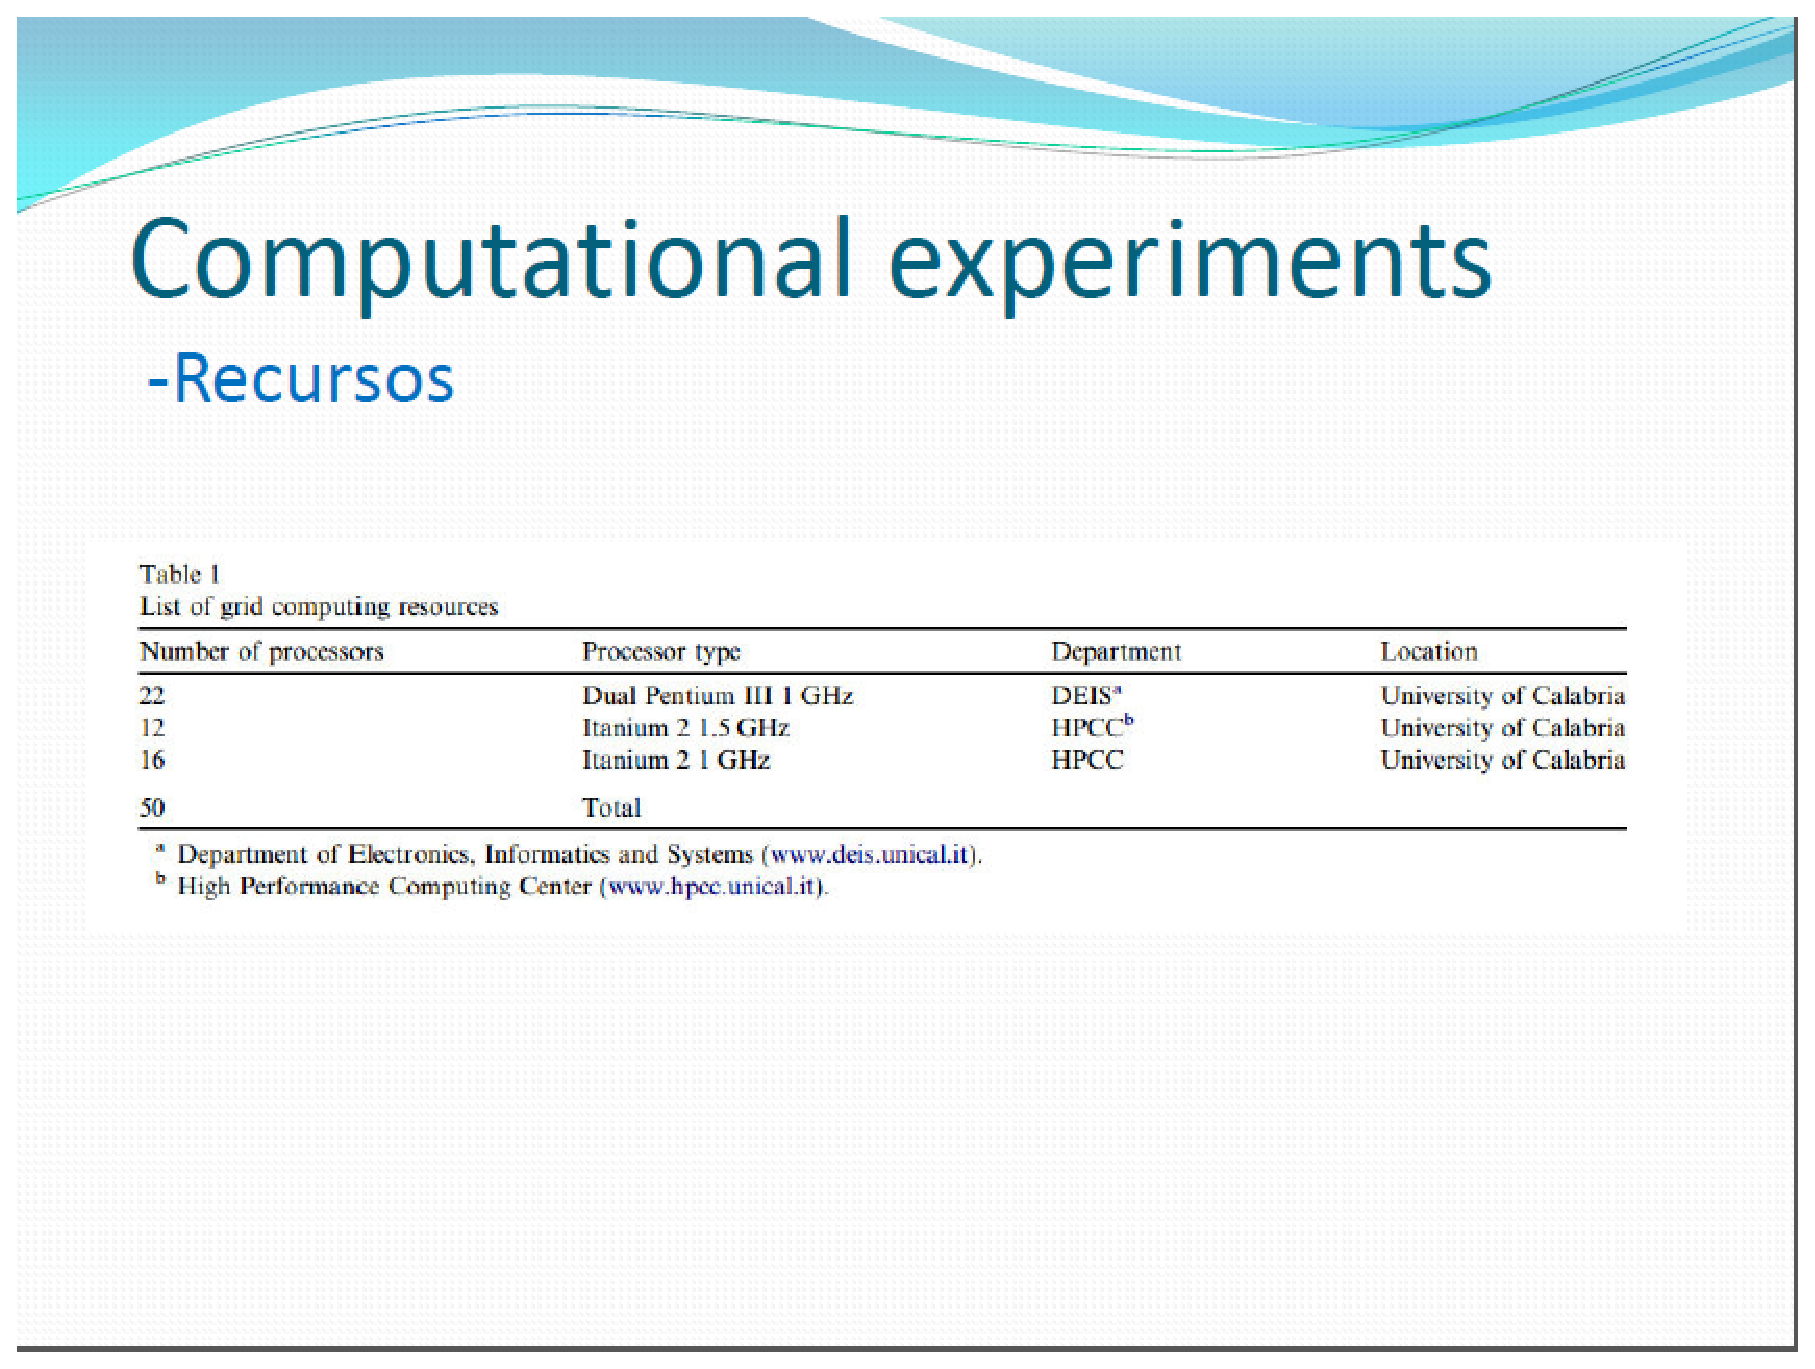
\includegraphics[width=1\textwidth]{images/pic13.eps}\\[0.25cm]
\end{center}
%%%%%%%%%%%%%%%%%%%%%%%%%%%%%%%%%%%%%%%%%%%%%%%%%%%%%%%%%%%%%%%%%%%%%%%%%%%%%%%
\begin{center}
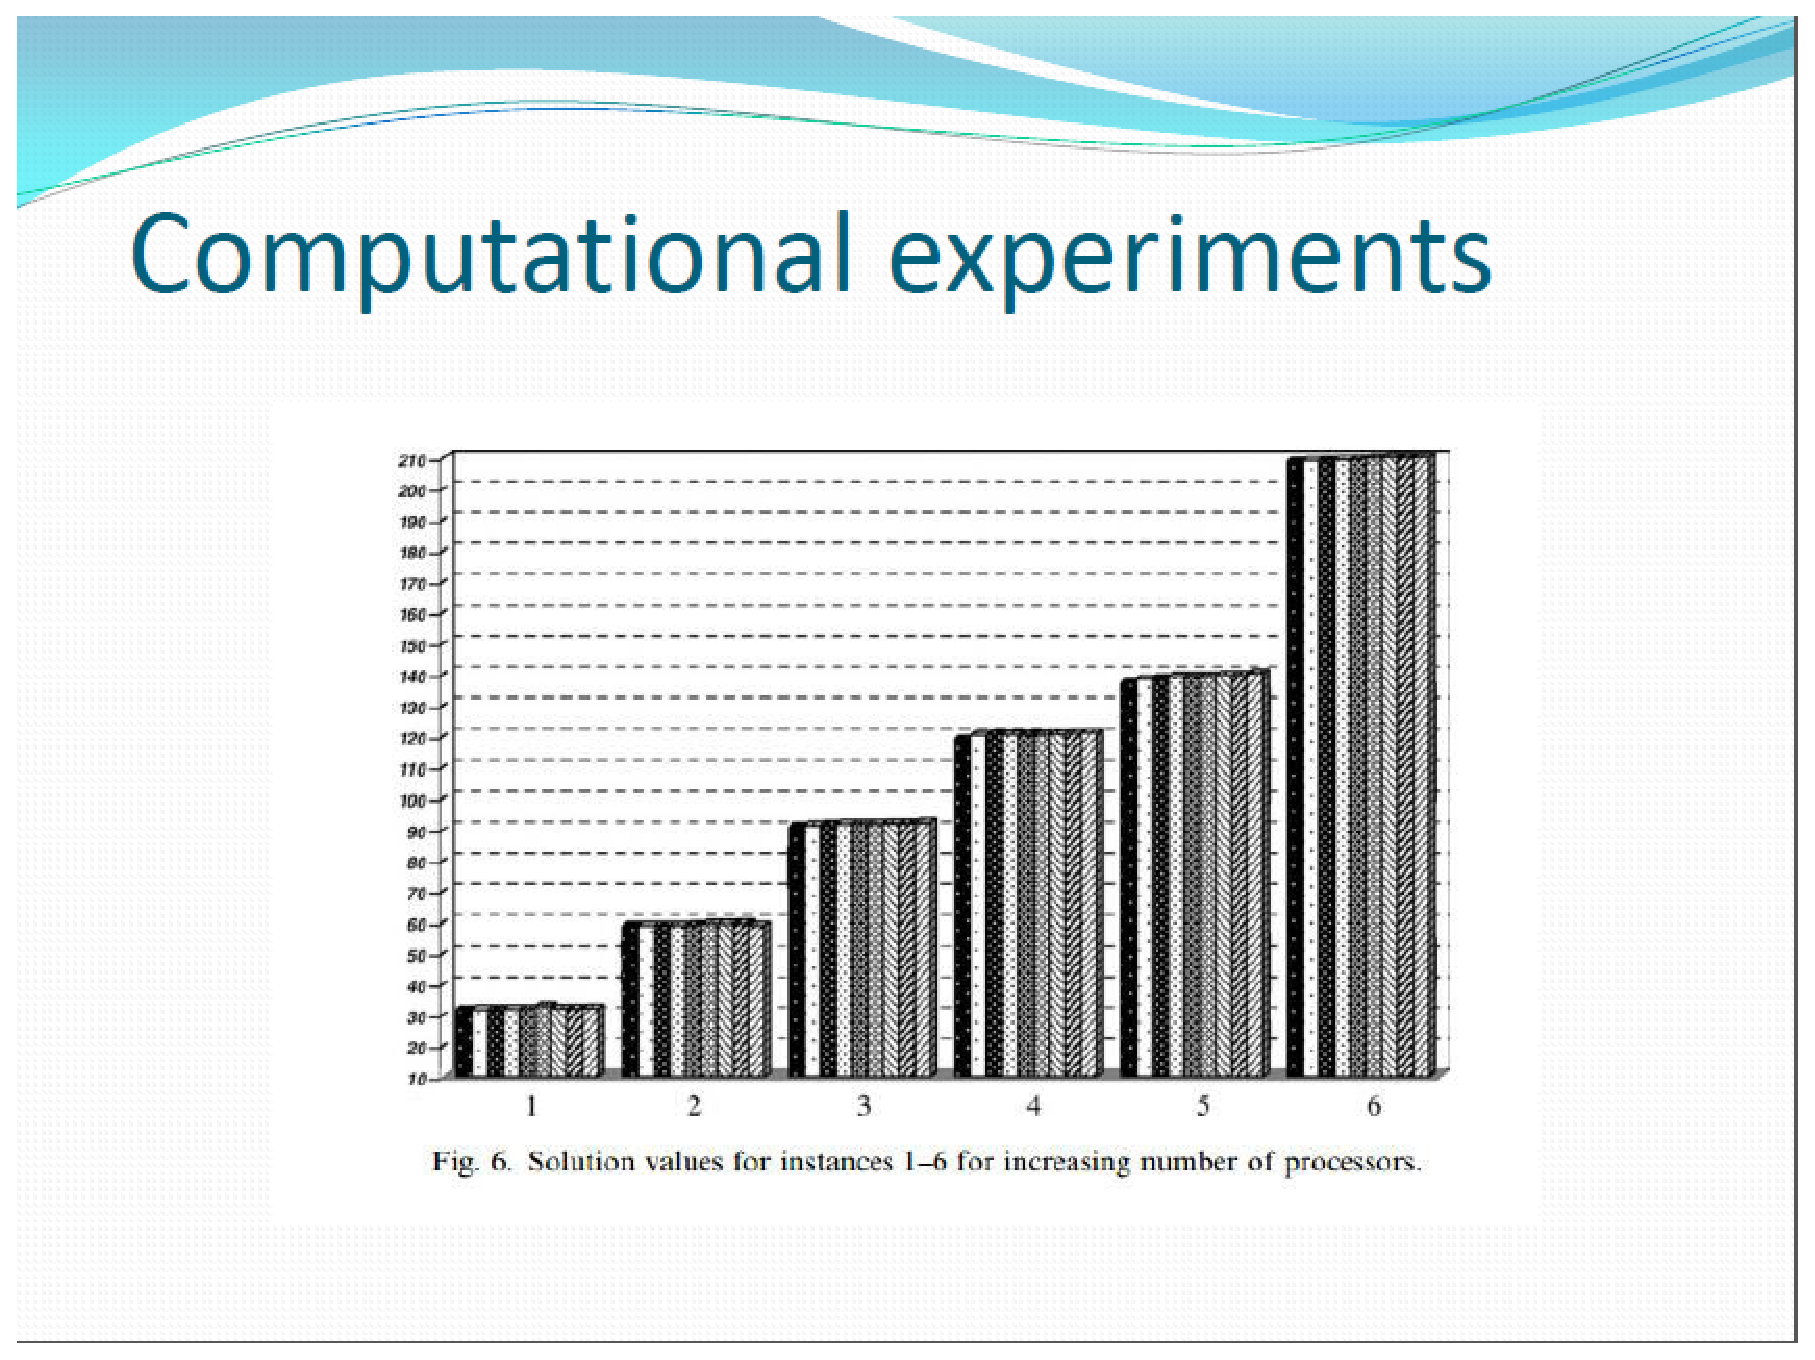
\includegraphics[width=1\textwidth]{images/pic14.eps}\\[0.25cm]
\end{center}
%%%%%%%%%%%%%%%%%%%%%%%%%%%%%%%%%%%%%%%%%%%%%%%%%%%%%%%%%%%%%%%%%%%%%%%%%%%%%%%
\thispagestyle{empty}
%\begin{appendix}

%\chapter{Título del Apéndice 1}
%\label{appendix:1}

%\input{tex/apendice1.tex}

%\chapter{Título del Apéndice 2}
%\label{appendix:2}

%\input{tex/apendice2.tex}

%\end{appendix}

%%%%%%%%%%%%%%%%%%%%%%%%%%%%%%%%%%%%%%%%%%%%%%%%%%%%%%%%%%%%%%%%%%%%%%%%%%%%%%%
\addcontentsline{toc}{chapter}{Bibliografía}
\bibliographystyle{plain}


\bibliography{bib/references}

\nocite{*}

%%%%%%%%%%%%%%%%%%%%%%%%%%%%%%%%%%%%%%%%%%%%%%%%%%%%%%%%%%%%%%%%%%%%%%%%%%%%%%%

\end{document}
